\documentclass[12pt]{article}

\usepackage{ctex}
\usepackage{geometry}
\usepackage{enumerate}
\usepackage{amsmath}
\usepackage{float}
\usepackage{subfigure} 
\usepackage{listings}
\usepackage{xcolor}
\usepackage{cases}
\usepackage{amssymb}    %triangleeq
\usepackage{lastpage}   %页码
\usepackage{fancyhdr}   %页眉页脚
\usepackage{graphicx}   %图片引用路径
\usepackage{indentfirst}    %缩进设置
\usepackage{booktabs}
\usepackage{multirow}

\setlength{\parindent}{2em}%缩进设置
\graphicspath{{C:/Users/adm/Desktop/课程文件/科学计算/作业/3.9作业/tex/image}}%图片引用Path,好像并没有什么用

%New colors defined below
\definecolor{codegreen}{rgb}{0,0.6,0}
\definecolor{codegray}{rgb}{0.5,0.5,0.5}
\definecolor{codepurple}{rgb}{0.58,0,0.82}
\definecolor{backcolour}{rgb}{0.95,0.95,0.92}

%Code listing style named "mystyle"
\lstdefinestyle{mystyle}{
  backgroundcolor=\color{backcolour},   commentstyle=\color{codegreen},
  keywordstyle=\color{magenta},
  numberstyle=\tiny\color{codegray},
  stringstyle=\color{codepurple},
  basicstyle=\ttfamily\footnotesize,
  breakatwhitespace=false,         
  breaklines=true,                 
  captionpos=b,                    
  keepspaces=true,                 
  numbers=left,                    
  numbersep=5pt,                  
  showspaces=false,                
  showstringspaces=false,
  showtabs=false,                  
  tabsize=2,
  language = python
}

%"mystyle" code listing set
\lstset{style=mystyle}
\usepackage{indentfirst}
\setlength{\parindent}{2em}%缩进设置

\graphicspath{{images/}}%图片引用Path
\geometry{left=1in,right=0.75in,top=1in,bottom=1in}     %页边距


\lhead{} %左上页眉

\begin{document}
\pagestyle{fancy}
\setcounter{page}{1}
\rhead{Page \thepage\ of \pageref{LastPage}}
%页码设置
\vspace{20pt}
\centerline{{\Large \textbf{计算机模拟 Homework6}}}
\vspace{15pt}

\centerline{{\large \textbf{汪奕晨 3180105843}}}
\vspace{15pt}

\centerline{{\large \textbf{数学科学学院 数学与应用数学专业}}}
\vspace{15pt}

%============================== Q1 =========================================
%============================= Problem Restatement =============================
\section{问题描述}
使用Monte-Carol积分计算
$$
    \int_0^1\frac{1}{2}\sin(\frac{1}{x^2}) + \frac{1}{2}
$$

并且在$\epsilon = 0.01, \delta = 0.01$的情况下使用chebyshev方法和norm-distribution方法计算所需的抽样次数。
%============================= Theory and Algorithms =============================
\section{设计思路}
通过equation (\ref{eq: chebyshev estimate},\ref{eq: norm estimate}) 可以分别用chebyshev方法和norm-distribution方法估计在给定$\epsilon, \delta$下所需的抽样次数。
其中$\Phi^{-1}$为标准正态分布逆函数,使用python实现时,可以调用scipy.stats.norm.ppf计算。

\begin{equation}
    n_c(\epsilon, \delta) = \lceil \frac{1}{4\delta\epsilon^2} \rceil
    \label{eq: chebyshev estimate}
\end{equation}

\begin{equation}
    n_n(\epsilon, \delta) =    \left\lceil \left[\frac{\Phi^{-1}(1 -\frac{\delta}{2})}{2\varepsilon}\right]^2\right\rceil.
    \label{eq: norm estimate}
\end{equation}


%============================= Results =============================
\section{模拟结果与分析}

chebyshev方法和norm-distribution方法估计的采样次数分别为$250000, 16384$, 我们采用$n=17000$进行测试

\begin{figure}[H]
    \centering
    \subfigure[Integral Curve]{
    \begin{minipage}[t]{0.4\linewidth}
    \centering
    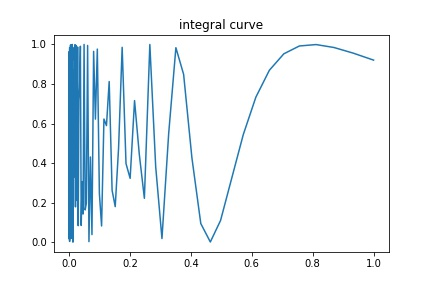
\includegraphics[width=7.5cm]{./figure/int_curve.jpg}
    \label{pic: integral curve}
    \end{minipage}
    }
    \subfigure[batch test resule when $N=17000, B=500$]{
    \begin{minipage}[t]{0.4\linewidth}
    \centering
    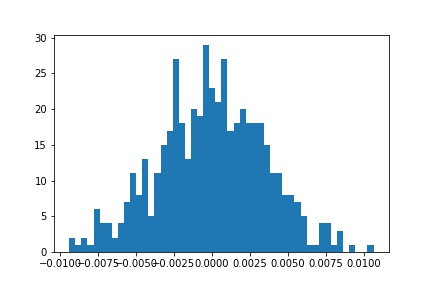
\includegraphics[width=7.5cm]{./figure/hist_n17000_b500.jpg}
    \label{pic: hist}
    \end{minipage}
    }
    \caption{Performance of Simulation}
    \label{pic: perf}
  \end{figure}

如Figure (\ref{pic: hist}), 只有少量的点落在误差$0.01$以外,考虑到测试了测试了500次,且要求的误差不超过0.01的概率为99\%,这些超过0.01的样本是可以接受的。

将500次计算的平均值作为计算结果,结果为$0.6431029411764705$
%============================= Conclution and Disscusion =============================
% \section{结论与进一步工作}


% %============================== Reference =====================================
% \addcontentsline{toc}{section}{References}

% \begin{thebibliography}{99}
%   %\bibliographystyle{unsrt}
%   % \bibliographystyle{unsrt}
%   \bibitem{Ref1}%temperature map
%   Global Climate Change: Evidence. (2019, October 24). Retrieved January 16, 2020, from https://neo.sci.gsfc.nasa.gov/view.php?datasetId=MYD28M
  
% \end{thebibliography}

% \nocite{*}
% \bibliographystyle{acm}
% \bibliography{test}
%================================ Appendix ========================================
\newpage
\section*{附录}
%============================= Codes =============================
\subsection*{代码}

\begin{lstlisting}
    # DEFINE
    EPS = 0.01
    DELTA = 0.01
    
    def func(x):
        return (1/2*np.sin(1/x/x) + 1/2)
    
    class MC_int():
        def __init__(self, func):
            self.func = func
    
    
        def plot_line(self, savepath = './tex/figure/int_curve.jpg'):
            x = np.logspace(-3,0,100)
            y = self.func(x)
            plt.figure()
            plt.plot(x, y)
            plt.title('integral curve')
            plt.savefig(savepath)
            plt.show()
    
    
        def integral(self, n):
            x = np.random.rand(n)
            y = np.random.rand(n)
            s = y < self.func(x)
            return sum(s)/n
    
    
        def batch_test(self, n, b):
            x = np.random.rand(b, n)
            y = np.random.rand(b, n)
            s = y < self.func(x)
            res = s.sum(axis = 1)/n
            # 下面的代码为上面的功能,但上面的代码向量化,速度更快
            # res = np.array([self.integral(n) for i in range(b)])
            m = res.mean()
            plt.figure()
            plt.hist(res-m, bins = 50)
            plt.savefig('./tex/figure/hist_n{}_b{}.jpg'.format(n,b))
            plt.show()
            return m
    
        @staticmethod
        def caln_chebyshev(eps, delta):
            return np.floor(1/4/delta/eps/eps)
    
        @staticmethod
        def caln_norm(eps, delta):
            return np.floor(norm.ppf(1-delta/2,loc=0,scale=1)/2/eps)**2
    
    
    MC = MC_int(func)

    n1 = MC.caln_chebyshev(EPS, DELTA)
    n2 = MC.caln_norm(EPS, DELTA)
    print(n1, n2)

    print(MC.batch_test(17000, 500))
\end{lstlisting}
\end{document}